\documentclass[11pt,spanish]{article}

% Paquetes
\usepackage{amstext}
\usepackage{amssymb}
\usepackage{amsmath}
\usepackage{babel}
    \addto\shorthandsspanish{\spanishdeactivate{~<>}}
    \decimalpoint
\usepackage[style=iso]{datetime2}
\usepackage{fancyhdr}
\usepackage{float}
\usepackage[T1]{fontenc}
\usepackage[a4paper]{geometry}
    \geometry{verbose,tmargin=3cm,bmargin=2cm,lmargin=2.5cm,rmargin=2.5cm}
\usepackage{graphicx}
\usepackage{hyperref}
\usepackage[utf8]{inputenc}
\usepackage{lastpage}
\usepackage{mathptmx}
\usepackage{tasks}
\usepackage{units}
\usepackage{siunitx}

% dibujos 

\usepackage{tikz}
\usepackage{tikz-dimline}
\usetikzlibrary{calc}
% \usetikzlibrary{math}
\usetikzlibrary{arrows.meta}
\usetikzlibrary{snakes}
\usetikzlibrary{decorations}
\usetikzlibrary{decorations.pathmorphing}
\usetikzlibrary{patterns}

% tipo de fuente 
\usepackage{lmodern}

\pagestyle{fancy}
\lfoot{\small DF, FCEyN, UBA}
\cfoot{\tiny Actualizado el {\today} a las {\DTMcurrenttime}}
\rfoot{\small Pág. {\thepage} de \pageref{LastPage}}

\begin{document}

% Título
    \begin{center}
    \textsc{\large Física 2 (Física) - Cátedra Diana Skigin}
    \par\end{center}{\large \par}
    
    \begin{center}
    \textsc{\large Segundo Cuatrimestre de 2021}
    \par\end{center}{\large \par}
    
    \begin{center}
    \textsc{\large Guía 6: Paquetes de Ondas}
    \par\end{center}{\large \par}

% Comienzo 
\begin{enumerate}

\section*{Velocidad de grupo y de fase}

% Ejercicio 1

    \item Discuta cuál de estos métodos permite determinar
    la velocidad de fase y cuál la de grupo:

    \begin{enumerate}
        \item Medir el tiempo que tarda un pulso sonoro (por ejemplo, un
        aplauso) en impactar sobre una superficie reflectora ubicada a una
        distancia conocida. y volver a su punto de partida.

        \item Medir la longitud de un tubo que resuena a una frecuencia conocida
        (y corregir por efectos de borde).

        \item Medir el tiempo que tarda un pulso lumínoso en recorrer una
        distancia conocida.

        \item Medir la longitud de una cavidad resonante que oscila en un
        modo y frecuencia conocidos.
    \end{enumerate}

% Ejercicio 2

    \item Obtenga la velocidad de fase y de grupo para los siguientes casos.
    Compárelas y discuta en cuales casos ambas velocidades son similares.
    
    \begin{enumerate}
        \item Ecuación de ondas clásica.
        \item Ecuación de Klein-Gordon, considerando las siguientes situaciones:
        \begin{enumerate}
            \item $\omega_0 = 0$, con $c$ y $k_0$ arbitrarios.

            \item $\omega_0 = \SI{1}{\per\second}$ y $c=\SI{1}{\meter\per\second}$,
            con $k_0$ tomando los valores: $\SI{1}{\per\meter}$,
            $\SI{3}{\per\meter}$, y $\SI{10}{\per\meter}$.
        \end{enumerate}
    \end{enumerate}

% Ejercicio 3

    \item Demuestre que la velocidad de grupo $v_\text{g}$ y la velocidad de fase
    $v_\text{f}$ están relacionadas por:
    \[
    v_\text{g}=v_\text{f}-\lambda\frac{dv_\text{f}}{d\lambda}
    \]
    ¿Cómo es $\frac{dv_\text{f}}{d\lambda}$ en un medio no dispersivo? En
    ese caso, ¿cómo se relacionan la velocidad de grupo y la de fase?


\section*{Paquetes Gaussianos}

% Ejercicio 4

    \item \textbf{Función Gaussiana:} Considere la siguiente función de una
    coordenada arbitraria $z$:
    \[
    f(z)=A\exp\left[-\frac{(z-\mu)^{2}}{4\Delta ^{2}}\right],
    \]
    conocida como función de Gauss (\textit{aka} campana de Gauss, función
    normal, etc.), cuyos parámetros $A$, $\mu$ y $\Delta$ son conocidos.
    
    \begin{enumerate}
        \item Muestre analítica o gráficamente que esta función:
        \begin{itemize}
            \item es definida positiva (si $A > 0$).
            \item tiene un único máximo en $z = \mu$.
            \item tiende a $0$ para $z \to \pm \infty$.
        \end{itemize}
 
        \item Determine el desplazamiento en $z$ respecto a la posición del
        máximo, necesario para que la altura de la función se reduzca a la
        mitad. Es decir, obtenga $\Delta z$ tal que:
        $$f(\mu \pm \Delta z)=\nicefrac{1}{2} f(\mu)$$
        Utilice este resultado para definir el ancho de la campana. ¿Qué
        parámetro de la función determina dicho ancho?
        
        \item ¿A qué altura de la función corresponde el ancho definido por
        $2 \Delta$?
    \end{enumerate}

% Ejercicio 5

    \item Se quiere investigar la relación entre el ancho de un paquete y el
    desfasaje de las frecuencias que lo componen.

    \begin{enumerate}

        \item Tome el siguiente pulso con un espectro gaussiano de ancho $\Delta k$
        centrado en $k_{0}$ (note que las frecuencias están en fase):
        \[
        \hat{\psi}(k)=A\exp\left[-\frac{(k-k_{0})^{2}}{4\Delta k^{2}}\right].
        \]
        Calcule $\psi(x)$ y vea que tiene una envolvente Gaussiana que modula
        una portadora de frecuencia $k_{0}$. Note que el pulso está centrado
        en $x=0$ y que se cumple la relación $\Delta x\Delta k=\nicefrac{1}{2}$
        (el paquete Gaussiano es el de mínima incerteza).

        \item Ahora desfase las distintas frecuencias en forma lineal, tal que:
        \[
        \hat{\psi}(k)=A\exp\left[-\frac{(k-k_{0})^{2}}{4\Delta k^{2}}\right]\exp\left[i\alpha(k-k_{0})\right].
        \]
        Calcule $\psi(x)$ y vea que es el mismo pulso que en la parte (a), pero
        desplazado en $\alpha$ hacia la derecha (una fase lineal sólo corre
        la función).

        \item Ahora agregue una fase cuadrática, es decir:
        \[
        \hat{\psi}(k)=A\exp\left[-\frac{(k-k_{0})^{2}}{4\Delta k^{2}}\right]\exp\left[i\beta(k-k_{0})^{2}\right].
        \]
        Calcule $\psi(x)$ y vea que es un pulso gaussiano centrado en $x=0$
        pero con un ancho $\Delta x$ que cumple:
        \[
        \Delta x\Delta k=\frac{1}{2}\sqrt{1+16\beta^{2}\Delta k^{4}}.
        \]
        
        Verifique que el producto de ambos anchos cumple la relación de
        incerteza general $\Delta x \Delta k \geq \nicefrac{1}{2}$, y luego
        determine el valor de $\beta$ tal que se cumpla la relación de mínima
        incerteza $\Delta x \Delta k = \nicefrac{1}{2}$.
        
        \item A partir del resultado anterior, discuta si es cierto que, si se
        quiere disminuir el ancho espacial de un paquete ($\Delta x$),
        \textit{siempre} se debe aumentar su ancho espectral ($\Delta k$).
        ¿Contradice esto a la relación de incerteza mínima?

        \textbf{Sugerencia:} Puede ser útil obtener $\Delta x$ como función de
        $\Delta k$, y luego graficar o derivar la primera en función de la
        segunda.

    \end{enumerate}

    \begin{description}
        \item [{Ayuda:}] $\int_{-\infty}^{+\infty}\exp\left[(x+a)^{2}\right]dx=\sqrt{\pi}$.
    \end{description}

% Ejercicio 6

    \item Repita el ejercicio anterior, considerando que el espectro
    $\hat{\psi}(k)$ corresponde a un pulso que se propaga en un medio arbitrario
    evaluado en $t=0$. Resuelva analíticamente a partir de la linealización de
    la relación de dispersión y halle $\psi(x,t)$ en cada caso. ¿Qué supuestos
    debe verificar el espectro para que el desarrollo sea lo más exacto posible?

% Ejercicio 7

    \item Se tiene un pulso de ancho $\Delta k$ centrado en $k_{0}$ tal que
    la siguiente es una buena aproximación para la relación de dispersión:
    \[
    \omega(k)=\omega_{0}(k_{0})+\omega'(k_{0})(k-k_{0})+\frac{1}{2}\omega''(k_{0})(k-k_{0})^{2}
    \]
    donde $\omega' = \frac{d \omega}{dk}$ y $\omega'' = \frac{d^2 \omega}{dk^2}$.
    Si en $t=0$ el pulso se propaga hacia $x<0$, y se escribe:
    \[
    \psi(x,0)=A\int_{-\infty}^{+\infty}\exp\left[-\frac{(k-k_{0})^{2}}{4\Delta k^{2}}\right]\exp\left(ikx\right)dk+ \text{c.c.},
    \]
    calcule $\psi(x,t)$. Obtenga la posición y el ancho del paquete
    como función del tiempo. ¿Es cierto que cualquier paquete se ensancha al
    viajar por un medio dispersivo?


\section*{Propiedades de la transformada de Fourier}    
    
% Ejercicio 8    
    
    \item Sea $f(t)$ una función real del tiempo. Muestre que su transformada de
    Fourier $\mathcal{F}[f]$ es una función de la frecuencia angular
    $\hat{f}(\omega)$  que cumple $\hat{f}(\omega)=\hat{f}(-\omega)$. Use esto
    para escribir a $f(t)$ como superposición de senos y cosenos.

% Ejercicio 9        

    \item Muestre que la transformada de Fourier $\mathcal{F}$ es una
    transformación lineal, es decir:
    \[
    \mathcal{F}[af+bg]=a\mathcal{F}[f]+b\mathcal{F}[g]
    \]
    donde $f$ y $g$ son funciones de $x$, y $a$ y $b$ son constantes.


\section*{Paquetes cuadrados}

% Ejercicio 10

    \item Considere un espectro de frecuencias cuadrado, centrado en una
    frecuencia angular $\omega_0$ y de ancho $\Delta\omega$:
    \begin{align}\hat{\phi}(\omega) =
        \begin{cases}
            \Delta\omega^{-1}, & \text{si } \omega \in [\omega_0 - \frac{\Delta\omega}{2}, \omega_0 + \frac{\Delta\omega}{2}] \\
            0, & \text{en caso contrario}
        \end{cases}
    \end{align}

    \begin{enumerate}
        \item Grafique el espectro $\hat{\phi}(\omega)$.
        
        \item Verifique que este espectro corresponde a una función $\phi(t)$
        dada por: 
        \[
        \phi(t)=\frac{1}{2\pi}\left[\frac{\sin(\tfrac{\Delta\omega}{2} t )}{\tfrac{\Delta\omega}{2} t}\right]e^{i\omega_{0}t}
        \]
        y grafique su módulo $\left|\phi(t)\right|$.

        \item Sea $T$ un tiempo más prolongado que la duración de cualquier
        experimento que pueda idear. Muestre que si $\Delta\omega$ es
        suficientemente pequeño como para que $\Delta\omega T\ll1$, entonces
        durante un tiempo menor que $T$, $\phi(t)$ es una función armónica de
        amplitud y fase prácticamente constantes. Elija valores numéricos razonables para $T$ y $\Delta \omega$, y grafique el espectro correspondiente.
    \end{enumerate}


% Ejercicio 11

    \item Considere una secuencia de pulsos de duración $\Delta t$ y amplitud
    $A_0$ que se repiten $N$ veces con período $\tau$ (con $\tau < \Delta t$),
    dando lugar a la siguiente señal $\phi(t)$:

    \begin{figure}[H]
        \centering{}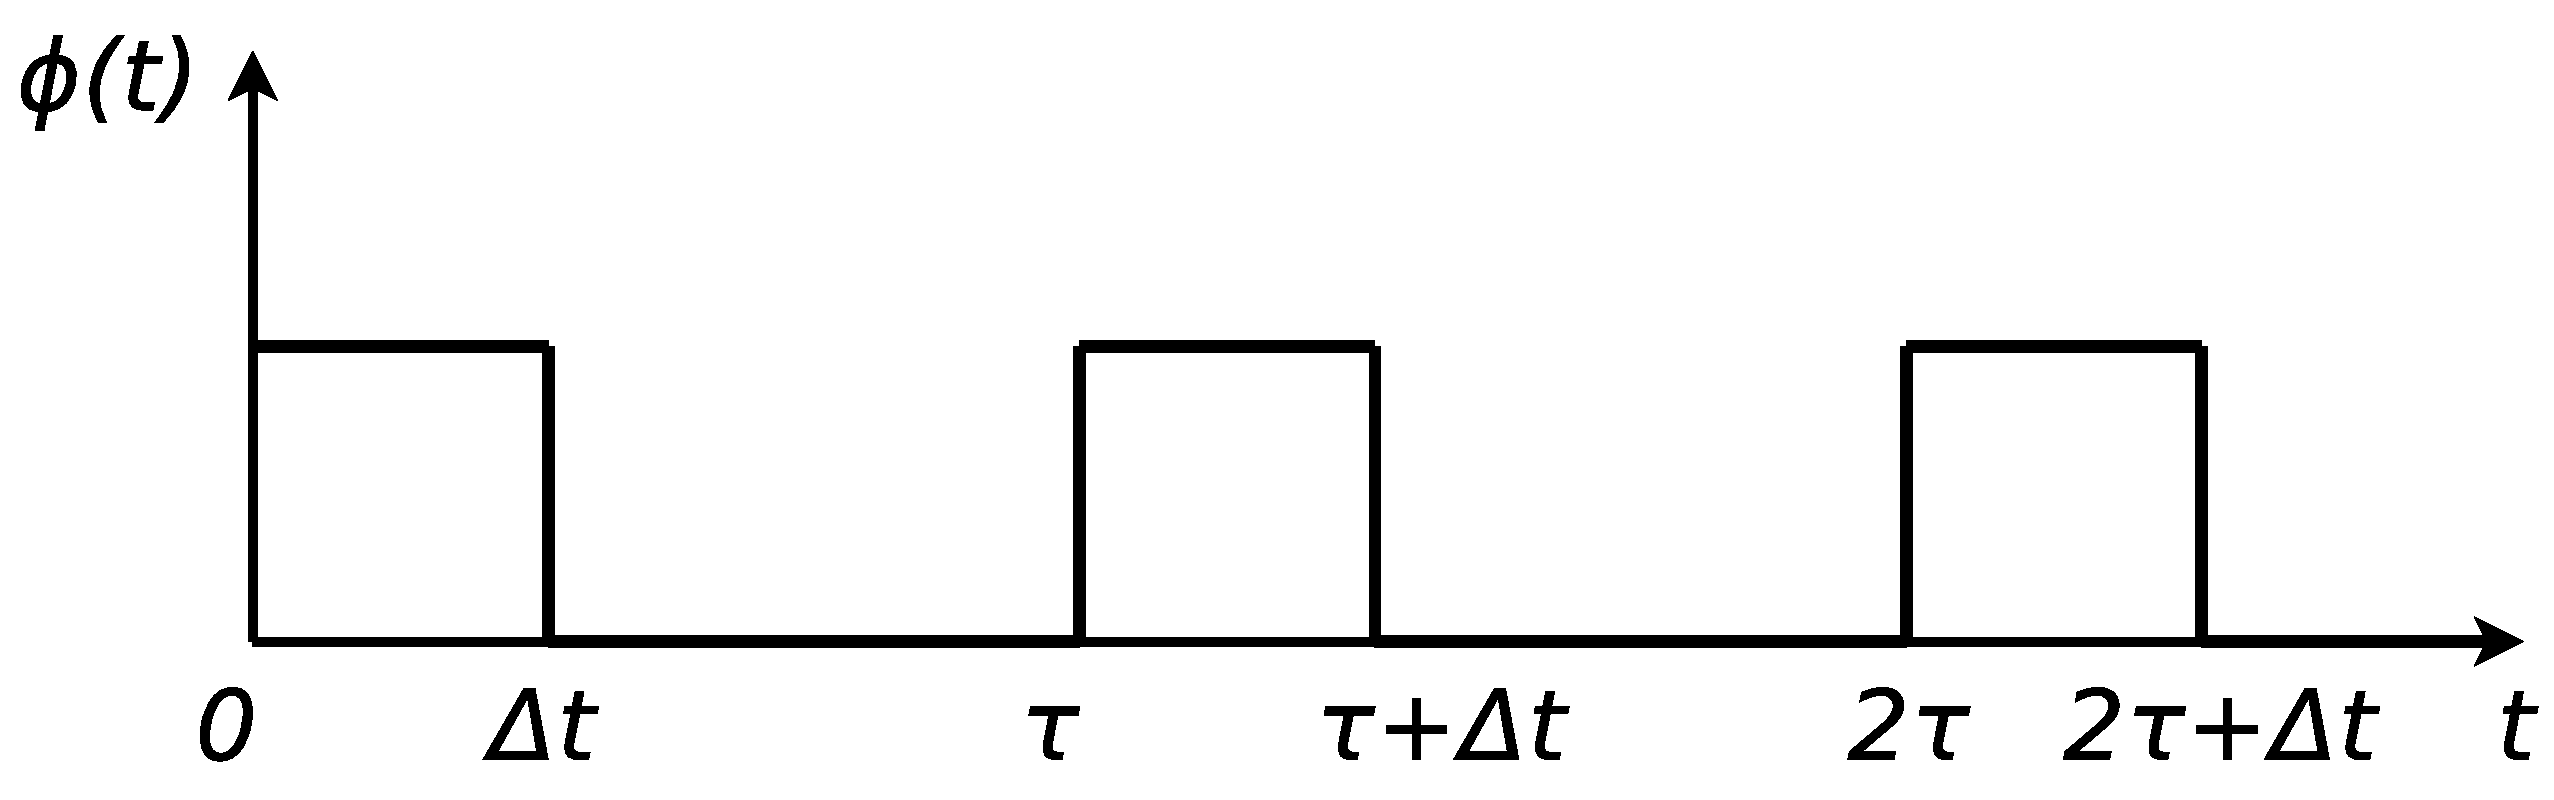
\includegraphics[clip,scale=0.25]{figs/ej2-18}
    \end{figure}

    \begin{enumerate}
        
        \item Considere la función que describe a un pulso situado en el
        intervalo $[n\tau, (n + 1)\tau]$:
        \begin{align}\phi_n(t) =
            \begin{cases}
            A_0, & \text{si } t \in [n\tau,n\tau+\Delta t ] \\
            0, & \text{en caso contrario}
            \end{cases}
        \end{align}
        de forma que $\phi(t) = \sum_{n=0}^{N-1} \phi_n(t)$. Compruebe que la
        transformada de $\phi_n(t)$ es igual a la transformada de $\phi_0(t)$,
        multiplicada por una fase $e^{i n \theta}$.
        
        \item Obtenga $\hat{\phi}_0(\omega)$ y a partir de la misma obtenga
        $\hat{\phi}(\omega)$.
        
        \item Considere la duración total de la señal $T_\text{tot}=N\tau$.
        Verifique que, para un valor finito de $T_\text{tot}$, el espectro
        $\hat{\phi}(\omega)$ está formado por una superposición de armónicos
        casi discretos de la frecuencia fundamental $\nu_{1}=\tau^{-1}$, siendo
        realmente cada armónico un continuo de frecuencias que se extiende sobre
        una banda de ancho $\Delta\nu\approx T_\text{tot}^{-1}$. Verifique
        también que los componentes armónicos más importantes se encuentran en
        el intervalo de frecuencias dado por $[0, \nu_\text{máx}]$, con
        $\nu_\text{máx} = \Delta t^{-1}$.

        \item ¿Por qué vale $\nu_\text{máx} \Delta t \approx1$ si, en principio,
        podría valer $\nu_\text{máx} \Delta t \gg 1$? ¿La misma pregunta es
        aplicable a $\Delta\nu$ y $T_\text{tot}$?
    \end{enumerate}


\section*{Propagación de paquetes en interfaces}

% Ejercicio 12

	\item Se tienen dos cuerdas semi--infinitas de distinta densidad lineal de
    masa, $\mu_{1}$ y $\mu_{2}$, unidas en un punto y sometidas a una tensión
    $T_0$. Sobre la primera, se propaga hacia la derecha una perturbación de la
    forma indicada en la figura, a velocidad $v$. Se conocen $\mu_{1}$,
    $\mu_{2}$, $T_0$, $L$ y $h$.

	\begin{figure}[H]
		\centering{}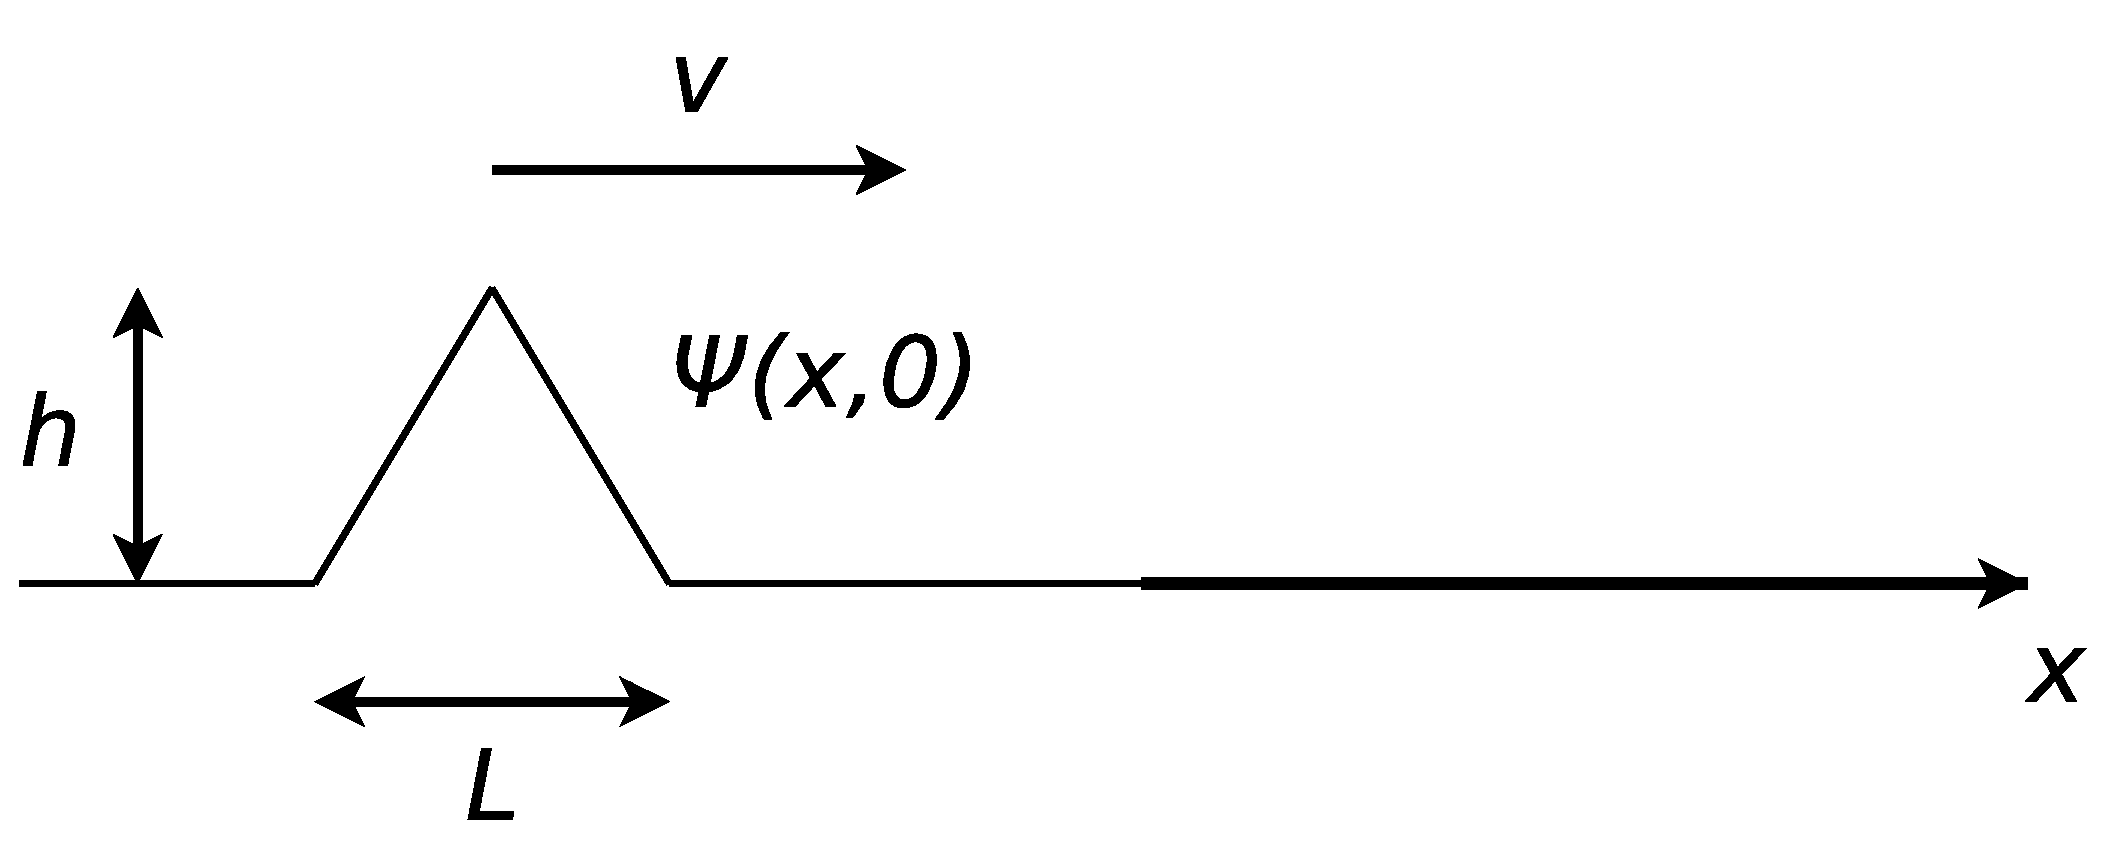
\includegraphics[clip,scale=0.25]{figs/ej2-20}
	\end{figure}

	\begin{enumerate}
		\item Hallar el desplazamiento $\psi(x,t)$ considerando que los medios
    	son no dispersivos.

		\item Explique cualitativamente cómo cambian estos resultados si el
        segundo medio es dispersivo.
	\end{enumerate}
    
\end{enumerate}

\end{document}
